\subsubsection{UC9 - Informazioni dettagliate funzione}
\begin{figure}[h]
	\centering
	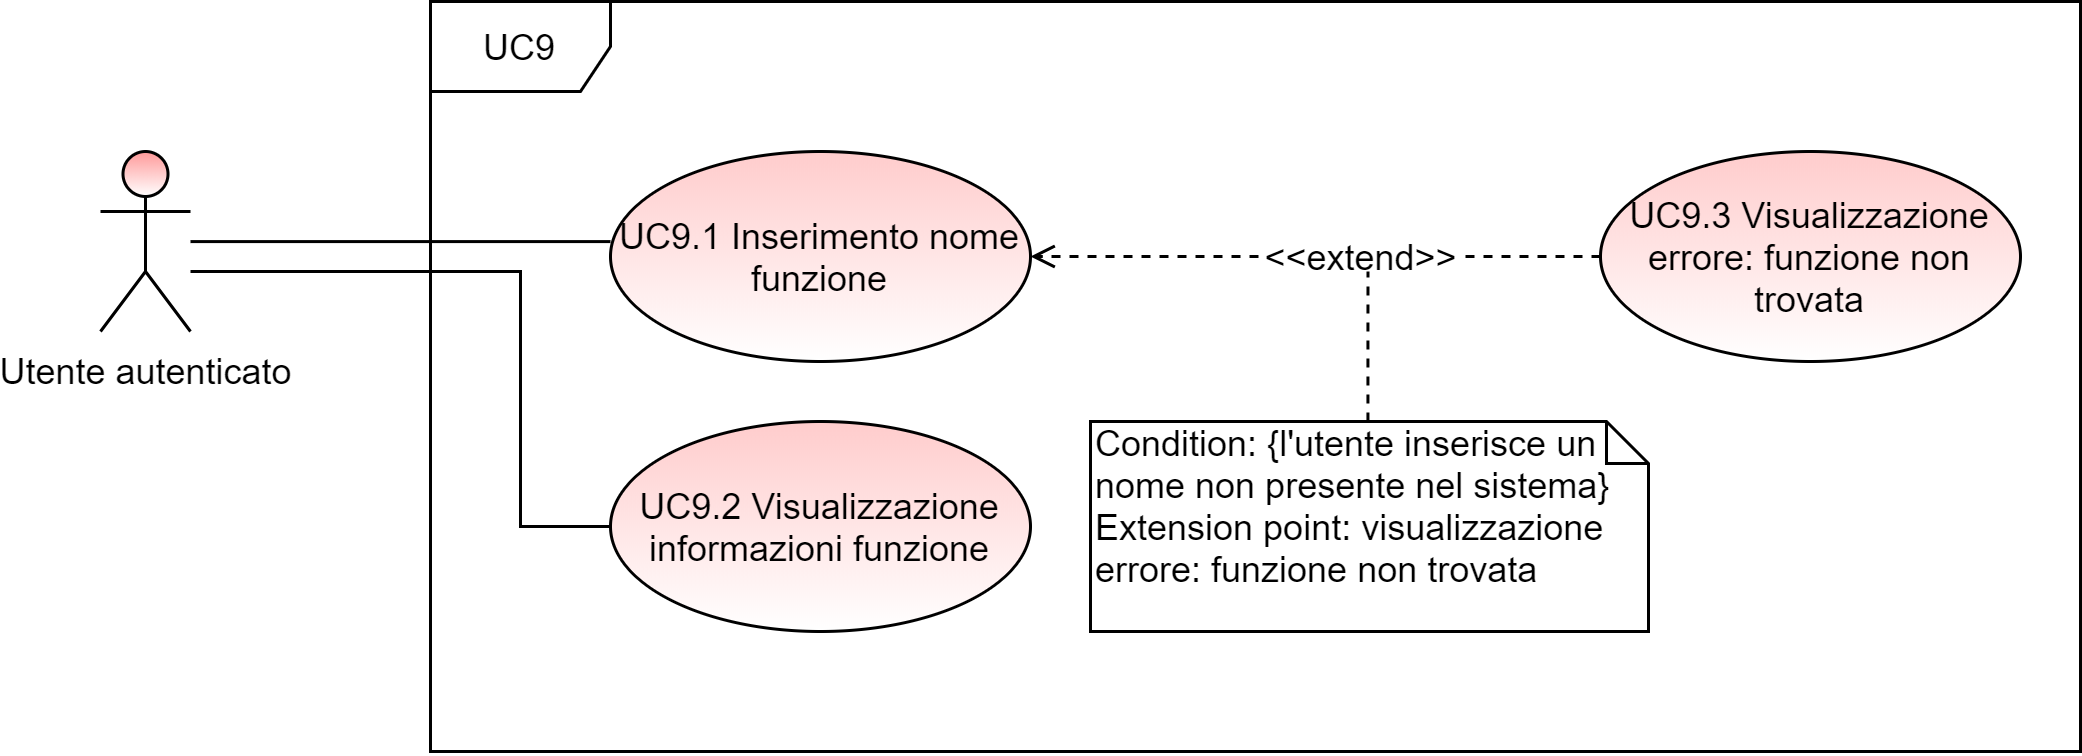
\includegraphics[scale=\ucs]{./res/img/UC9.png}
	\caption {UC9 - Informazioni dettagliate funzione}
\end{figure}
\begin{itemize}
	\item \textbf{Attori primari:} \ua{};
	\item \textbf{Attori secondari:} \re{};
	\item \textbf{Descrizione:} l’utente richiede la visualizzazione della descrizione completa di una funzione di cui conosce il nome eseguendo il comando \pinfo{}. Il sistema riporta le informazioni relative a tale funzione;
	\item \textbf{Scenario principale:} 
	\begin{itemize}
		\item l'utente richiede di visualizzare le informazioni dettagliate di una funzione tramite il comando \pinfo{}; 
		\item vengono visualizzate le informazioni relative alla funzione in questione.
	\end{itemize}
	\item \textbf{Precondizione:} l'utente inserisce correttamente ed esegue il comando \pinfo{};
	\item \textbf{Postcondizione:} la CLI\ped{\textit{G}} riporta la descrizione completa della funzione in questione.
\end{itemize}